\graphicspath{{img/algor/}}
\chapter{Algoritmos}

\section{Ejemplos}
\subsection{Ordenamiento de una lista de valores en orden ascendente-Algoritmo de la burbuja}
Supongamos que se tiene el vector
\[\begin{bmatrix}
  A_1 &A_2 &A_3 & \cdots &A_N
\end{bmatrix}\]
de orden $N$ y se desea organizarlo en orden ascendente. En el denominado 
algoritmo de la burbuja\footnote{Ver 
\url{https://en.wikipedia.org/wiki/Bubble_sort}.} se hacen recorridos del 
vector en los cuales se comparan pares de valores consecutivos y se hacen las 
permutaciones que sean necesarias de acuerdo con el resultado de la 
comparación. El ordenamiento termina cuando se haga una pasada por el vector 
sin la necesidad de realizar ninguna permutación.

\begin{algorithm}[H]
\SetAlgoLined
\KwData{Vector A de orden N}
\KwResult{Vector original con elementos en orden ascendente}
READ $N$\;
READ $A_i$\;
\Repeat{$NSW=0$}{
    $i \leftarrow 1$ \;
    $NSW \leftarrow 0$ \;
    \While{$i<N$}{
        \If{${A_i} > {A_{i + 1}}$}{
            SWAP(${A_i},{A_{i + 1}}$)\;
            $NSW \leftarrow NSW+1$\;
        }
        $i \leftarrow i+1$\;
    }
}
\caption{Algoritmo de la burbuja}
\label{bubble}
\end{algorithm}

Nótese que en el algoritmo de la burbuja hemos usado la función SWAP($A$,$B$) la cual se encarga de realizar el intercambio de los valores almacenados en las variables $A$ y $B$. La función SWAP se define en el siguiente algoritmo.

\begin{algorithm}[H]
  \SetAlgoLined
  \KwData{Numbers to swap A, B}
  \KwResult{A and B with changed values}
  $temp \leftarrow A$\;
  $A \leftarrow B$\;
  $B \leftarrow temp$\;
\caption{Función SWAP($A$,$B$)}
\label{swap}
\end{algorithm}

\subsection{Ordenamiento de una lista de valores en orden ascendente-Algoritmo de selección}
En este algoritmo se recorre el vector original $N$ veces y en cada pasada se extrae el valor mínimo y la posición del valor mínimo. Esto se ilustra en la siguiente estructura matricial en la cual la primera fila corresponde al vector original (con los valores en desorden). El valor mínimo en cada fila se muestra resaltado en negrilla. En cualquier caso la fila $i+1$ corresponde a la fila $i$ tras haber extraído el valor mínimo.
\[\begin{bmatrix}
  \bf{1} &5 &3 &2 &7 &4\\
  5 &3 &\bf{2} &7 &4 &0\\
  5 &\bf{3} &7 &4 &0 &0\\
  5 &7 &\bf{4} &0 &0 &0\\
  \bf{5} &7 &0 &0 &0 &0\\
  7 &0 &0 &0 &0 &0
\end{bmatrix}\]

Posteriormente el valor mínimo se acomoda en el vector solución. En la siguiente secuencia se muestra la forma del vector solución tras cada iteración.
\begin{align*}
&\begin{bmatrix}
  1 &0 &0 &0 &0 &0
\end{bmatrix}\\
&\begin{bmatrix}
  1 &2 &0 &0 &0 &0
\end{bmatrix}\\
&\begin{bmatrix}
  1 &2 &3 &0 &0 &0
\end{bmatrix}\\
&\begin{bmatrix}
  1 &2 &3 &4 &0 &0
\end{bmatrix}\\
&\begin{bmatrix}
  1 &2 &3 &4 &5 &0
\end{bmatrix}\\
&\begin{bmatrix}
 1& 2 &3 &4 &5 &7
\end{bmatrix}
\end{align*}

A continuación se presenta el algoritmo de inserción. En este haremos uso del concepto de función. En programación una función no es otra cosa que un programa, que procesa datos de entrada para producir resultados o datos de salida, pero que esperamos usar de manera repetida en varios programas diferentes. En la definición (o declaración) de una función es importante distinguir cuales son los datos de entrada y cuales son los datos de salida. Para esto adoptaremos la siguiente convención

\begin{algorithm}[H]
 \SetAlgoLined
 \KwData{$n$ input parameters}
 \KwResult{$k$ output results}
 Instr-1\;
 Instr-2\;
 ...\;
 Instr-n\;
\caption{function\_name($Par-1$,..,$Par-n$;$Res-1$,...,$Res-k$)}
\label{seqstru}
\end{algorithm}

En esta \texttt{function\_name} corresponde al nombre de la función y entre paréntesis se declaran o definen los parámetros o datos de entrada y los resultados o datos de salida. En la definición de la función estos parámetros se separan por un punto y coma (;).

En el algoritmo de selección definiremos 2 funciones. La primera llamada MINOR se encargará de extraer el menor valor de un vector y su posición, mientras que la segunda se encarga de copiar la fila $i$ en la fila $i+1$ tras haber extraído el valor mínimo. La definición de estas funciones se deja como tarea. El algoritmo de inserción tiene entonces la siguiente forma

\begin{algorithm}[H]
\SetAlgoLined
\For{$j\leftarrow i$ \KwTo $N$}{\nllabel{forins}
    MINOR($A_{ij}$; $min$, $ipos$)\;
    $R_i \leftarrow min$\;
    EXTRACT($A_{ij}$, $ipos$; $A_{i+1j}$)\;
}
\caption{Selection algorithm}
\label{algo:selection}
\end{algorithm}


\subsection{Organización de un vector fila en una matriz}
Suponga que se tiene un total de $N \times M$ datos correspondientes a la aceleración del terreno y registrada mediante acelerógrafos localizados en $N$ sitios diferentes de la ciudad. Cada registro contiene un total de $M$ datos de aceleración para $M$ datos de tiempo. Sin embargo la totalidad de los datos se encuentra almacenada en un arreglo unidimensional (o vector) de orden $N \times M$ donde cada grupo de $N$ datos corresponde a las aceleraciones en un mismo instante de tiempo para las $N$ estaciones. Con el fin de procesar el registro para cada estación se requiere extraer la información y almacenarla en una matriz de orden $N \times M$  en la cual cada fila corresponde a las aceleraciones registradas en una misma zona de la ciudad.

El siguiente algoritmo presenta un algoritmo para almacenar el vector en una matriz. En este caso, se almacena una fila de la matriz en cada iteración.\\
\begin{algorithm}[H]
\SetAlgoLined
\KwData{Vector $V$  of order $N\times M$}
\KwResult{Matrix of order $\left[ N, M \right]$}
READ $N$\;
READ $M$\;
READ $V$\;
\For{$i \leftarrow 1$ to $N$}{
	$Mat \left[ i, : \right] \leftarrow V \left[1+N \left( i-1 \right), N i \right]$;	
}
\caption{Escritura de un vector en una matriz. Opción 1}
\label{matrix}
\end{algorithm}


El siguiente algoritmo también presenta un algoritmo para almacenar el vector en una matriz. En este caso, se almacena una posición de la matriz en cada iteración. Note los dos ciclos anidados, mientras en el caso anterior se usó un único ciclo.\\
\begin{algorithm}[H]
\SetAlgoLined
\KwData{Vector $V$  of order $NxM$}
\KwResult{Matrix of order $\left[ N, M \right]$}
READ $N$\;
READ $M$\;
READ $V$\;
\For{$i \leftarrow 1$ to $N$}{
	\For{$j \leftarrow 1$ to $M$}{
		$Mat \left[ i, j \right] \leftarrow V \left[ i+N \left( j-1 \right) \right]$;	
	}
}
\caption{Escritura de un vector en una matriz. Opción 2}
\label{matrix}
\end{algorithm}


\subsection{Numeros primos}
En esta sección presentamos algunos algoritmos relacionados con números primos. El primer algoritmo verifica si un número entero dado es primo o no y devuelve un mensaje con esta información.\\
\begin{algorithm}[H]
\SetAlgoLined
 \KwData{number N}
 \KwResult{Prime or no-prime number}
READ $N$\;
$iflag \leftarrow 0$ \;
\For{$i\leftarrow 2$ \KwTo $N-1$}{\nllabel{forins}
  \If{$n \mod i = 0$}{
    $iflag \leftarrow 1$;
  }
}
\eIf{$iflag = 0$}{
  WRITE ``Prime number''\;
}{
  WRITE ``No-prime number''\;
}
\caption{Prime number verification}
\label{algo:primos}
\end{algorithm}

Una vez contemos con un algoritmo para verificar si un número es primo o no
podemo realizar la descomposición en factores primos para cualquier número
entero mayor a 2. El siguiente algoritmo presenta cómo hacerlo.\\
\begin{algorithm}[H]
\SetAlgoLined
 \KwData{number N}
 \KwResult{Prime factors of a number N}
READ $N$\;
\For{$i\leftarrow 2$ \KwTo $N$}{\nllabel{forins}
  $res\leftarrow n \mod i$ \;
  \If{$res = 0$}{
    Detect if i is prime ($iflag = 0$)\;
    \If{$iflag=0$}{
    WRITE ``Is prime''\;
    }
  }
}
\caption{Prime factors of a number}
\label{algo:primos_factores}
\end{algorithm}

El siguiente algoritmo presenta el pseudocódigo para encontrar la suma de todos
los primos menores que cierto número $N$ dado.\\
\begin{algorithm}[H]
\SetAlgoLined
\KwData{number N}
\KwResult{Sum of all the primes up to N}
READ $N$\;
$sum \leftarrow 2$ \;
\For{$i\leftarrow 3$ \KwTo $N$}{\nllabel{forins}
    Detect if i is prime ($iflag = 0$)\;
    \If{$iflag=0$}{
        $sum \leftarrow sum +i$\;
    }
}
\caption{Sum of the prime numbers up to a given value}
\label{algo:primos_suma}
\end{algorithm}

\subsection{Mallador de dominios rectangulares}
En una gran cantidad de métodos numéricos como diferencias finitas, elementos finitos, elementos de frontera se requiere de la partición o división del dominio del problema en sub-dominios o elementos. Algunos ejemplos se muestran en la \cref{fig:meshes}.
\begin{figure}[H]
\centering
    \begin{subfigure}[t]{0.48\textwidth}
		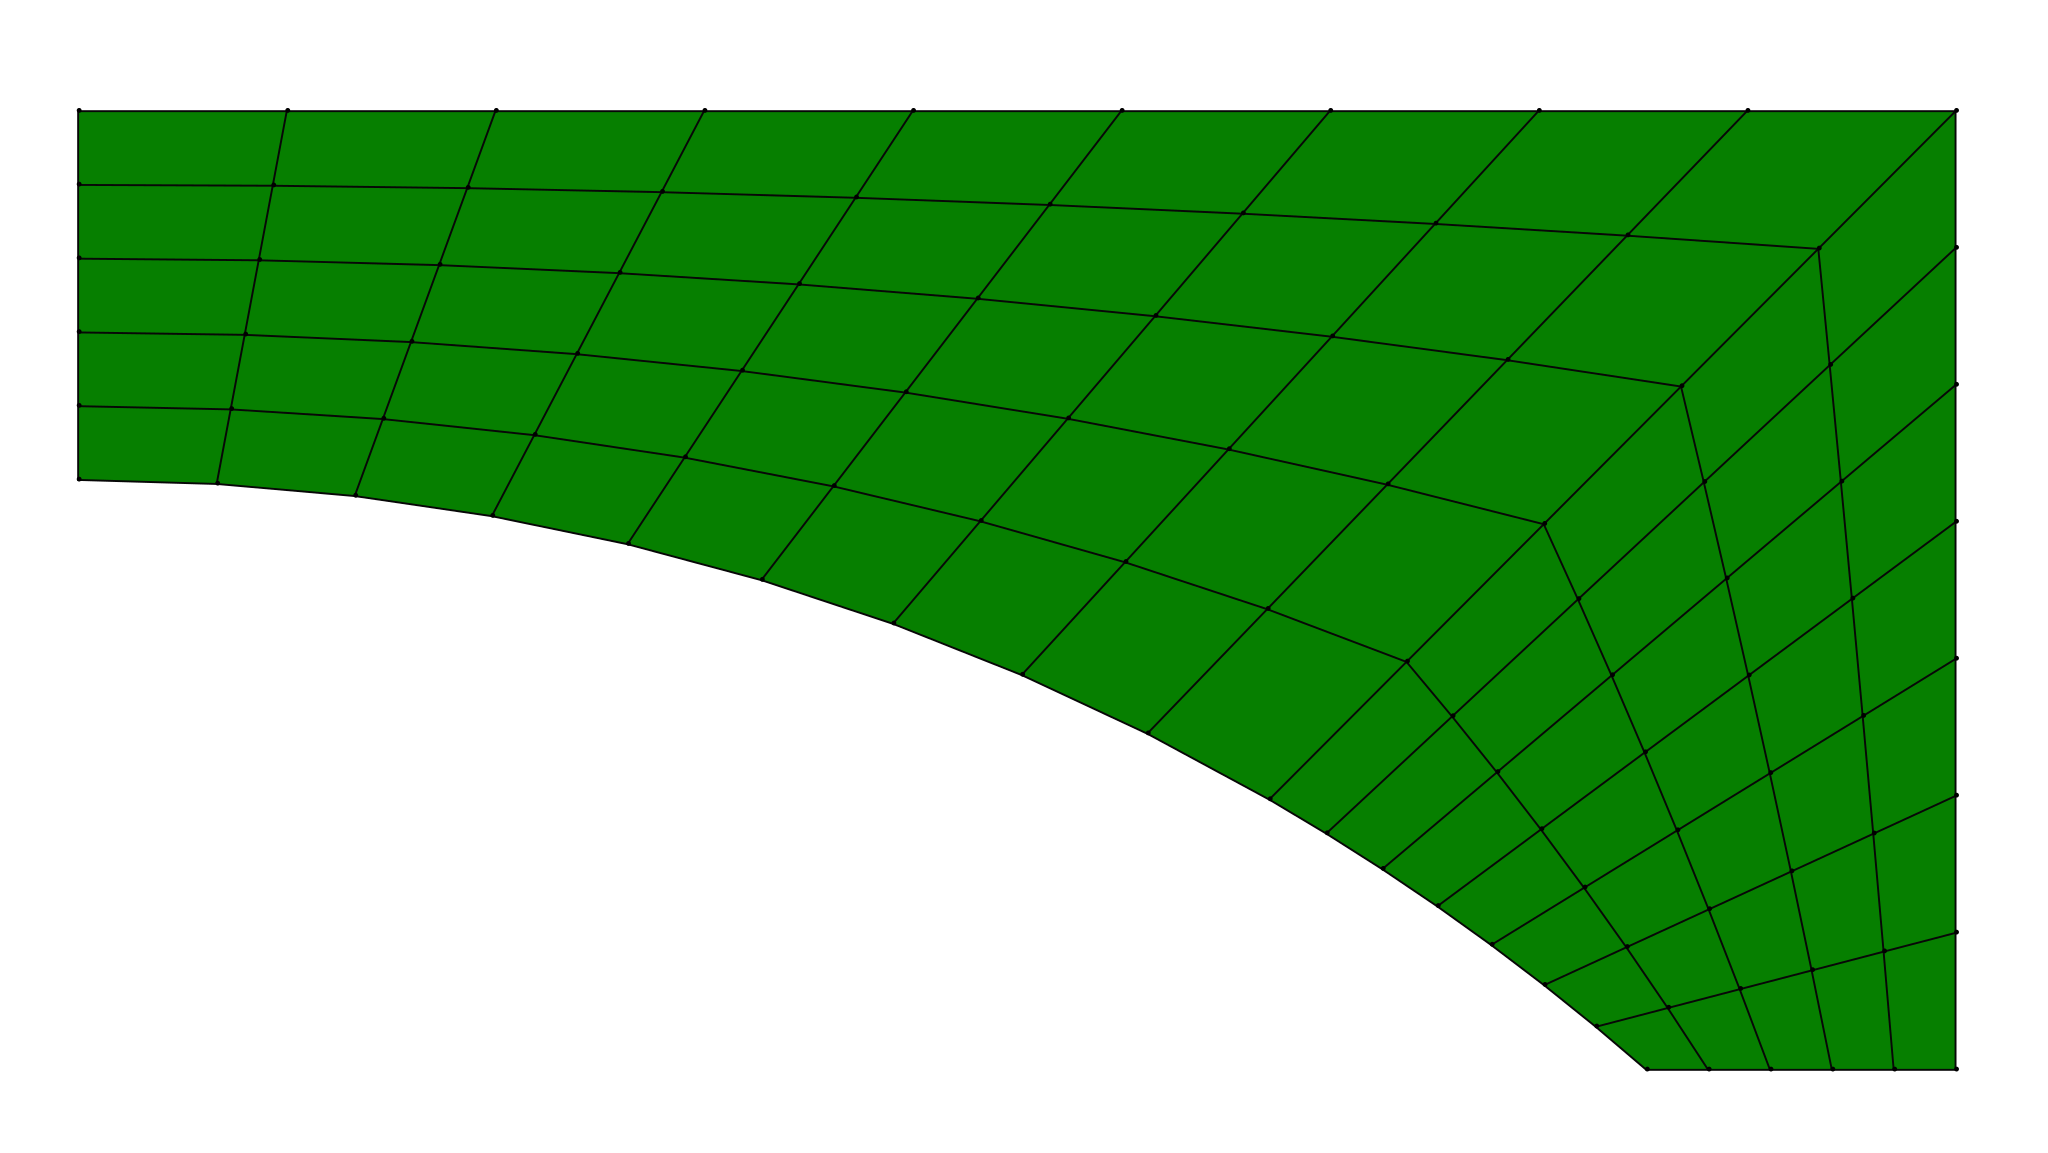
\includegraphics[width=\textwidth]{Mesh_bridge.pdf}
		\caption{}
	\end{subfigure}\,
    \begin{subfigure}[t]{0.35\textwidth}
		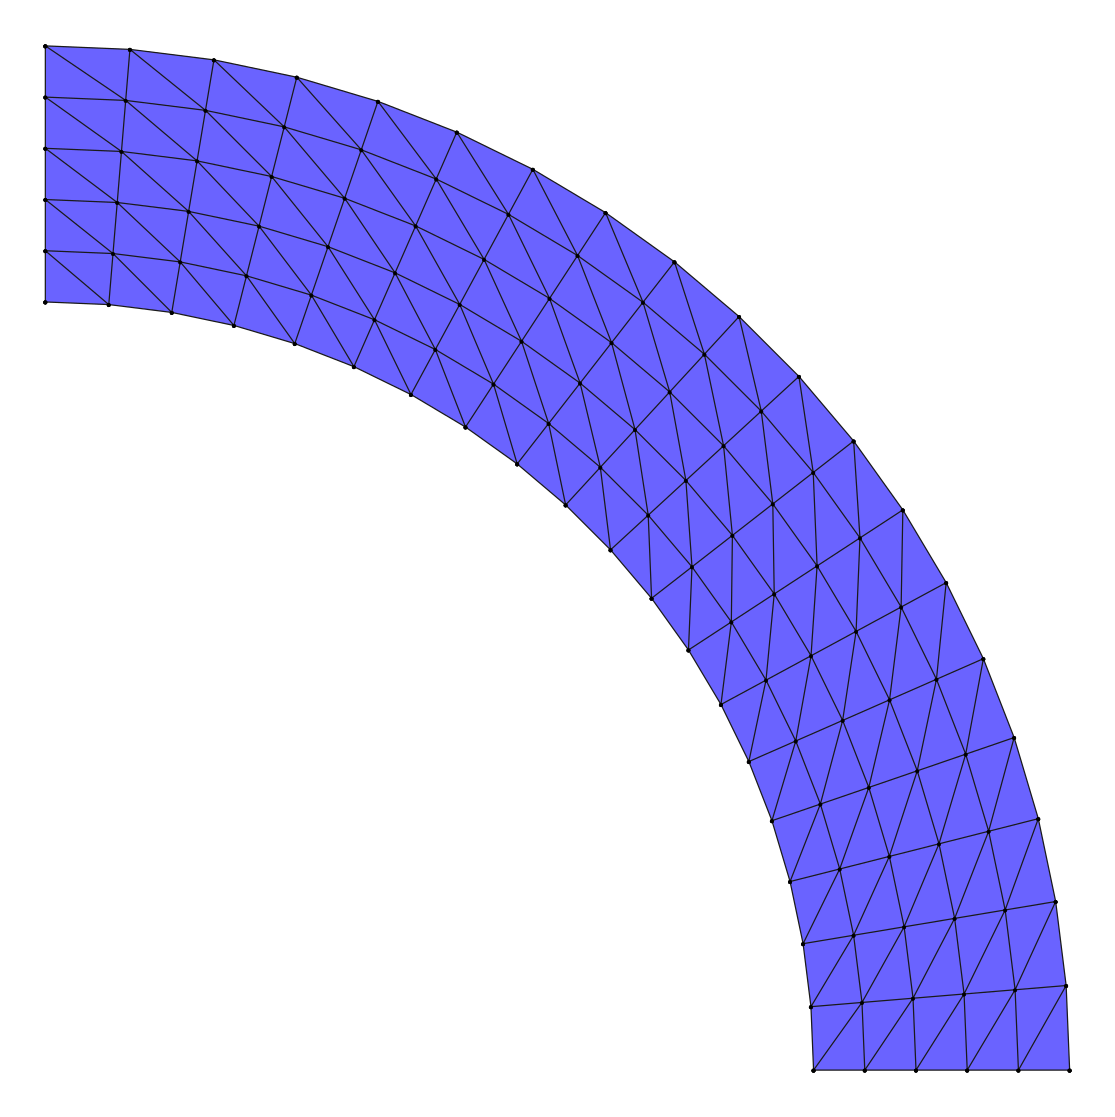
\includegraphics[width=\textwidth]{Mesh_ring.pdf}
		\caption{}
	\end{subfigure}
\caption{Mallas para el análisis de un puente y una tubería por medio del método de los elementos finitos. En el primer caso el dominio del problema esta dividido en subdominios de 4 lados mientras que la tubería se dividió en elementos triangulares.}
\label{fig:meshes}
\end{figure}

Este tipo de particiones se denominan mallas. Generalmente una malla corresponde a una serie de sub-dominios o elementos definidos por un determinado numero de puntos (o nudos) y por los puntos mismos. Por ejemplo, las mallas de los problemas ilustrados en la \cref{fig:meshes} están conformadas por elementos de 4 y de 3 lados que resultan de unir 4 y 3 puntos respectivamente.

En los programas de Mecánica Computacional un elemento se define mediante la declaración de un número entero, correspondiente al identificador del elemento, y el listado de puntos o nodos que conforman el elemento.
\begin{figure}[H]
\centering
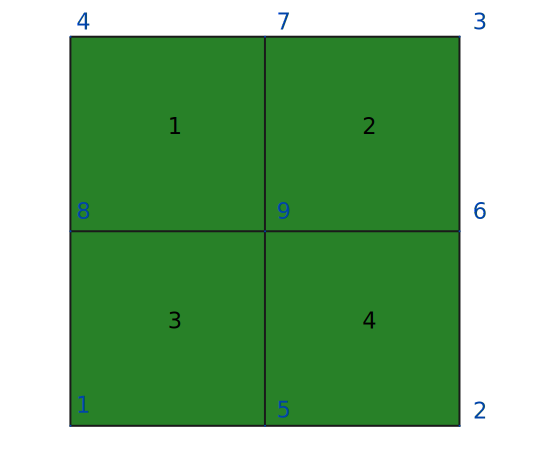
\includegraphics[width=0.50\textwidth]{Mesh_quad.pdf}
\caption{Malla de un dominio cuadrado dividido en 4 subdominios cuadrados.}
\label{fig:quad}
\end{figure}


Por ejemplo, considere el elemento 1 de la malla mostrada en la \cref{fig:quad}. Este se define como se ilustra en la \cref{fig:eledef}. En esta, el primer entero corresponde al identificador del elemento, mientras que los 4 enteros subsiguientes corresponden a los identificadores de los 4 nudos que conforman el elemento.
\begin{figure}[H]
\centering
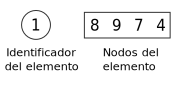
\includegraphics[width=2 in]{mesh_element_def.pdf}
\caption{Definición de un elemento cuadrado correspondiente al identificador del elemento y 4 nudos.}
\label{fig:eledef}
\end{figure}

En el proceso de creación de una malla es necesario definir el orden que deben seguir los puntos que conforman un elemento. Dicha definición se hace en términos de un elemento típico o generalizado. Por ejemplo, el ordenamiento de los nudos del elemento $1$ corresponde a un ordenamiento de un elemento típico como el que se muestra en la \cref{fig:tipico}. Nótese que este elemento se encuentra definido por sus 4 nodos y el sentido en el que estos están relacionados.
\begin{figure}[H]
\centering
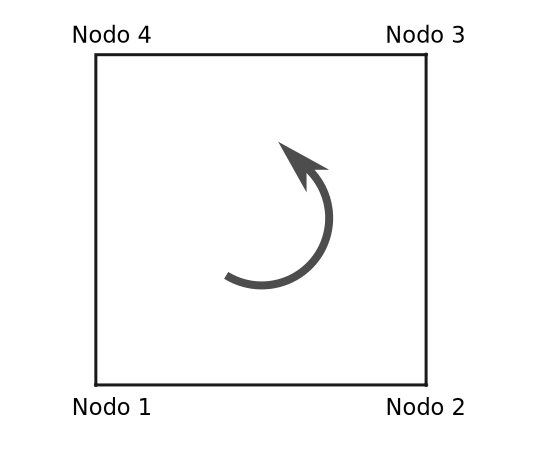
\includegraphics[width=0.50\textwidth]{mesh_tipico.pdf}
\caption{Definición de un elemento típico en el que se declara el ordenamiento de los nodos.}
\label{fig:tipico}
\end{figure}

\pagebreak
\subsection{Ejemplo: Algoritmo para mallado de dominios rectangulares}
Considere el dominio rectangular de ancho $W$ y altura $H$ dividido en 18 subdominios cada uno de ellos correspondiente a un elemento de 4 lados definidos por los 4 nudos que se muestran en \cref{fig:full}. Definiendo como $\Delta x$ y $\Delta y$ los tamaños característicos en las direcciones $X$ y $Y$ respectivamente diseñar un algoritmo que genere la malla para un dominio rectangular como el mostrado en la figura.
\begin{figure}[H]
\centering
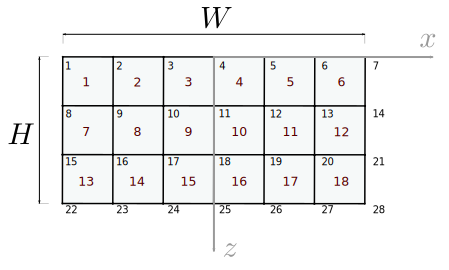
\includegraphics[width=5 in]{malla_algor.pdf}
\caption{Dominio rectangular.}
\label{fig:malla_algor}
\end{figure}

El archivo de datos correspondiente al caso particular del dominio mostrado en la \cref{fig:malla_algor} se muestra a continuación.
\begin{center}
\begin{minipage}[t]{0.3\textwidth}
\texttt{archivo\_puntos.txt}
\small
\begin{verbatim}
1  -3.0   0.0
2  -2.0   0.0
3  -1.0   0.0
4   0.0   0.0
5   1.0   0.0
6   2.0   0.0
7   3.0   0.0
8  -3.0   1.0
9  -2.0   1.0
10 -1.0   1.0
11  0.0   1.0
12  1.0   1.0
13  2.0   1.0
14  3.0   1.0
15 -3.0   2.0
16 -2.0   2.0
17 -1.0   2.0
18  0.0   2.0
19  1.0   2.0
20  2.0   2.0
21  3.0   2.0
22 -3.0   3.0
23 -2.0   3.0
24 -1.0   3.0
25  0.0   3.0
26  1.0   3.0
27  2.0   3.0
28  3.0   3.0
\end{verbatim}
\end{minipage}
\begin{minipage}[t]{0.3\textwidth}
\texttt{archivo\_elementos.txt}
\small
\begin{verbatim}
1    1   2   9   8
2    2   3  10   9
3    3   4  11  10
4    4   5  12  11
5    5   6  13  12
6    6   7  14  13
7    8   9  16  15
8    9  10  17  16
9   10  11  18  17
10  11  12  19  18
11  12  13  20  19
12  13  14  21  20
13  15  16  23  22
14  16  17  24  23
15  17  18  25  24
16  18  19  26  25
17  19  20  27  26
18  20  21  28  27
\end{verbatim}
\end{minipage}
\end{center}


\begin{algorithm}[H]
\SetAlgoLined
\KwData{Domain dimensions $W$ and $H$ and characteristic element sides ${\Delta x}$ and ${\Delta y}$ along the $x$ and $y$ directions; Horizontal coordinate of the left-most point $x_L$}
\KwResult{Text files containing the nodal point coordinates and element connectivities}
READ $W$, $H$, ${\Delta x}$, ${\Delta y}$, $x_L$ \;
$Mx \leftarrow W/\Delta x$ (number of elements in $x$);\\
$My \leftarrow H/\Delta y$ (number of elements in $y$);\\
$Nx \leftarrow Mx+1$ (number of points in $x$);\\
$Ny \leftarrow My+1$ (number of points in $y$);\\
$l \leftarrow 0$;\\
\For{$j \leftarrow 1$ to $Ny$}{
    \For{$i \leftarrow 1$ to $Nx$}{
        $l \leftarrow l+1$;\\
        $x \leftarrow {x_L} + (i - 1) \cdot \Delta x$;\\
        $y\leftarrow (j - 1) \cdot \Delta y$;\\
        WRITE to point file: $l$, $x$, $y$
    }
}
$l \leftarrow 0$ (for elements);\\
$q \leftarrow 0$ (for node-1);\\
$k \leftarrow 0$ (for node-3);\\
\For{$i \leftarrow 1$ to $My$}{
    $q \leftarrow q+1$;\\
    $k \leftarrow q+Nx+1$;\\
    \For{$j \leftarrow 1$ to $Mx$}{
        $l \leftarrow l+1$;\\
        WRITE to element file: $l$, $q$, $q+1$, $k$, $k-1$;\\
        $q \leftarrow q+1$;\\
        $k \leftarrow k+1$;\\
    }	
}
\caption{Mesher for simple rectangular domains}
\label{lineal}
\end{algorithm}




